\chapter{Instrukcja obs�ugi}
\label{cha:insObs}

%---------------------------------------------------------------------------
\section{Pobieranie aplikacji}
\label{sec:oobieranieAplikacji}

Aplikacje nale�y pobra� ze strony alloysvisualisation.codeplex.com (po prawej stronie znajduje si� przycisk Download). W skompresowanym pliku znajduje si�:
\begin{enumerate}%[1)]
\item Plik wykonywalny ComplexAlloysVisualisation.exe
\item skrypt chmcMergeScript.py
\item biblioteka WPFExtensions.dll
\item folder out
\end{enumerate}

Plik ComplexAlloysVisualisation.exe startuje aplikacj�. 

\section{Tworzenie modelu i manipulacja}
\label{sec:modelManipulacja}

Po uruchomieniu aplikacji nale�y nacisn�� przycisk Open File i wybra� plik .chmc. W folderze out znajduje si� klika przyk�adowych plik�w. Aplikacja domy�lnie stworzy model z serii 14. Aby zmieni� serie, nale�y nacisn�� przycisk Mask i w panelu po prawej stronie wybra� interesuj�ce nas serie.  W rozdziale 4.3 Graficzny Interface U�ytkownika znajduje si� dok�adny opis ka�dej funkcjonalno�ci.

\section{Przetwarzanie grupy plik�w}
\label{sec:przetwarzanie}

W celu przetworzenia grupy plik�w, nale�y uruchomi� aplikacje i nacisn�� przycisk Process Files. Po naci�ni�ciu pojawi si� okno, gdzie nale�y wybra� folder z plikami .chmc.

\begin{figure}[h!]
  \centering
	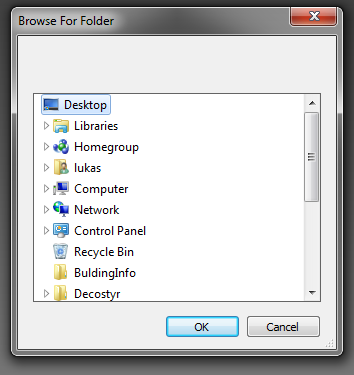
\includegraphics[scale=0.6]{process}
	\caption{Okno wyboru folderu.}
\end{figure}

\newpage

Przetwarzanie plik�w przy kliku seriach powinno trwa� oko�o 0,6 s dla ka�dego pliku. Wyniki zapisane zostan� w folderze screens. 

